% begin module inverse-function-equations
\begin{frame}
Let $f$ be a one-to-one function.
\[
\alert<handout:0| 4>{f^{-1}(y) = x} \qquad \Leftrightarrow \qquad \alert<handout:0| 3>{f(x) = y} .
\]
\uncover<2->{Therefore
\[
(f^{-1}\circ f)(x) = f^{-1}(\alert<handout:0| 3>{f(x)}) = \uncover<3->{\alert<handout:0| 4>{f^{-1}(\alert<handout:0| 3-4>{y})}} \uncover<4->{\alert<handout:0| 4>{ = x}.}
\]
}
\uncover<5->{
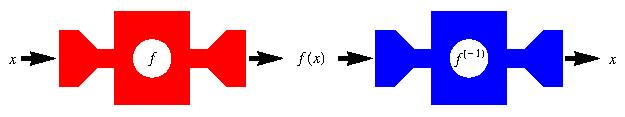
\includegraphics[height=2cm]{inverse-functions/pictures/07-01-machinesb.pdf}%
}

\uncover<6->{Therefore
\[
(f\circ f^{-1})(y) = f(\alert<handout:0| 7>{f^{-1}(y)}) = \uncover<7->{\alert<handout:0| 8>{f(\alert<handout:0| 7-8>{x})}} \uncover<8->{\alert<handout:0| 8>{ = y}.}
\]
}
\uncover<9->{
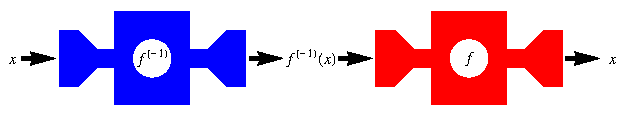
\includegraphics[height=2cm]{inverse-functions/pictures/07-01-machinesa.pdf}%
}
\end{frame}
% end module inverse-function-equations
